%==============  code_only_box.tex  =================
\documentclass[11pt]{article}

% 레이아웃/폰트 (필요 없으면 빼도 됨)
\usepackage{geometry}
\geometry{margin=1in}
\usepackage{fontspec}
\usepackage[space]{xeCJK}          % ← minted와의 verbatim 충돌 피하려면 [space] 옵션은 쓰지 마세요
\setCJKmainfont{Noto Sans KR}

\usepackage{setspace}
\setstretch{1.2}
\setlength{\parindent}{0pt}
\setlength{\parskip}{6pt}


% tcolorbox + (minted|listings) 토글
\newif\ifuseminted
\usemintedtrue             % minted 사용(하이라이트 예쁨). 안 되면 false로 바꿔 listings 사용

\usepackage[many]{tcolorbox}
\tcbuselibrary{skins,breakable,listings,minted}
\usepackage{xcolor}
\definecolor{codebg}{RGB}{248,248,248}
\usepackage{enumitem}          % ★ 필요
\usepackage{graphicx}
\usepackage{float}
% --- minted 버전: "코드 전용" 박스 (listing only)
\ifuseminted
  \usepackage{minted}       % 컴파일: xelatex -shell-escape code_only_box.tex
  \newtcblisting{CodeBox}[1][]{
    enhanced, breakable,
    colback=codebg, frame hidden,
    boxrule=0pt, borderline={0.5pt}{0pt}{black!15, dashed},
    sharp corners, before skip=8pt, after skip=12pt,
    listing engine=minted,
    listing only,            % ★ 박스 안엔 오직 코드만
    minted language=python,  % 필요 시 \begin{CodeBox}[minted language=c++] 로 덮어쓰기
    minted options={
      fontsize=\small,
      breaklines,
      autogobble,
      linenos,
      numbersep=6pt,
      tabsize=2
    },
    #1                       % 사용자 옵션 전달
  }
\else
% --- listings 버전: shell-escape 불가 시
  \usepackage{listings}
  \lstdefinestyle{mylist}{
    basicstyle=\ttfamily\small,
    numbers=left, numbersep=6pt,
    breaklines=true,
    tabsize=2,
    backgroundcolor=\color{codebg},
    showstringspaces=false
  }
  \newtcblisting{CodeBox}[1][]{
    enhanced, breakable,
    colback=codebg, frame hidden,
    boxrule=0pt, borderline={0.5pt}{0pt}{black!15, dashed},
    sharp corners, before skip=8pt, after skip=12pt,
    listing engine=listings,
    listing only,            % ★ 박스 안엔 오직 코드만
    listing options={style=mylist, language=Python},
    #1
  }
\fi



\begin{document}

\begin{center}
  {\LARGE \bfseries Graph based Block Digonalization 코드 주석 정리} \\[10pt]
  {\large 최윤호}
\end{center}

\section{분자(화합물) 정의}
\begin{CodeBox}[title={Example: Python snippet}]
geometry = [('H', (0., 0., 0.)),
            ('H', (dist, 0., 0. )),
            ('H', (2*dist, 0., 0. )),
            ('H', (3*dist, 0., 0.))]  # Angstrom
basis = 'sto-3g'
mol = MolecularData(geometry, basis, multiplicity=1, charge=0)
# qiskit 의 molecularinfo 와 같이 분자의 정보를 담고있는 클래스를 생성 이때 필요한 정보는 기하학적인 구조(geometry), basis, 시스템의 multiplicity와 총 전하량 등의 정보가 필요하다. 
\end{CodeBox}

\begin{enumerate}[label=\textbf{*}, leftmargin=*]
  \item geometry : 원자의 종류와 기하학적인 구조를 튜플로써 저장 ('원소종류', (x,y,z))
  \item basis : 전자의 atomic orbital 을 표현할 basis 설정 (sto3g, 6-31g,$\cdots$)
  \item MolecularData: qiskit 의 molecularinfo 와 같이 분자의 정보를 담고있는 클래스
\end{enumerate}
이는 객체는 분자(화합물)의 정보를 담고있는 객체로써, 이후 이 객체로부터 전자의 개수나, scf 계산을 수행할것이다. 
이번 논문에서 사용한 화합물은 H2 Cluster 로써 아래와같이 모든 수소원자가 같은 거리만큼 떨어져있는 구조를 의미한다. 
\begin{figure}[h]
    \centering
    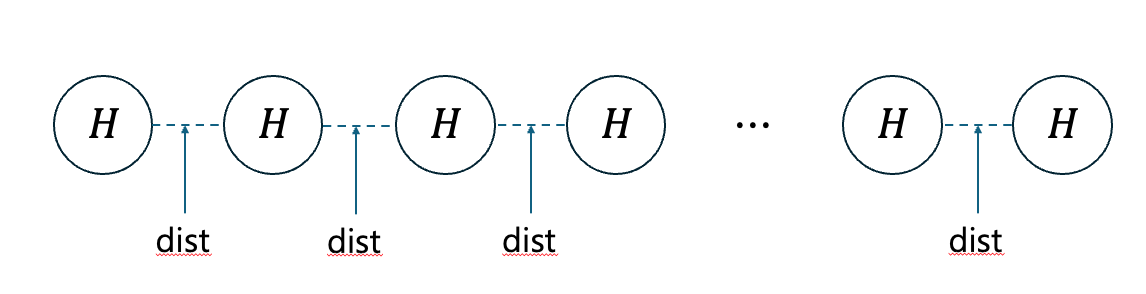
\includegraphics[width=0.8\textwidth]{/Users/choeyunho/Documents/mygit/2025_GBBD/실험코드_주석정리/fig/h2cluster.png}
    \caption{H2 Cluster}
    \label{fig:my_image}
\end{figure}


\section{FCI 행렬 생성}
\begin{CodeBox}[title={Example: Python snippet}]
mol = run_pyscf(mol_input, run_scf=1, run_fci=0)
# mol_input : 앞서 MolecularData 클래스를 이용해 생성된 객체 분자의 여러 정보를 담고있다. 
# run_pyscf : mol_input 을 바탕으로 계산을 수행 2nd Quantized 헤밀토니안을 얻기위한 HF 계산을 수행한다. 
# 이때 옵션으로 여기서 FCI 계산을 수행할수도 있으나, 이는 Cost가 매우커서 수행하지 않는다. 
ham_int = mol.get_molecular_hamiltonian()
# pyscf 계산을 수행한 이후 정보를 담고있는 mol 이라는 객체로 부터 1차/2차 적분에 대한 정보를 가져온다. 
# (*) 이후 객체 정보에 대한 추가설명
ham_fci = get_fermion_operator(ham_int)
# 1차/2차 적분에 대한 정보를 담고있는 ham_int로 부터 2nd Quantized된 헤밀토니안을 가져온다. 
# (**) 이후 객체 정보에 대한 추가설명 

H = get_number_preserving_sparse_operator(
# 전자수 와 스핀량 보존을 포함하는 FCI 행렬을 만들기 위한 함수
fermion_op=ham_fci, #사용할 2nd Quantized 헤밀토니안
num_qubits=mol.n_qubits, #총 스핀오비탈 개수 openFermion 패키지에서는 이를 qubit 라는 이름으로 사용하지만, 같은 의미.
num_electrons=mol.n_electrons,  # 시스템의 전자수 
spin_preserving=True)        # 시스템의 multiplicity가 보존되는 Determinant 만을 사용
H_real = H.real # 행렬의 각 원소는 두 Determinant로 기술되는 내적이며 이는 에너지에 대응되는 값이므로 실수값을 갖게되므로, 이후 그래프 연산을 위해 실수로 변환
# (***) 이후 객체 정보에 대한 추가설명 
\end{CodeBox}
\newpage
\subsection{(*) mol.get\_molecular\_hamiltonian()}
1차, 2차 적분의 결과를 아래와같이 저장 한다. 
\begin{figure}[H]
    \centering
    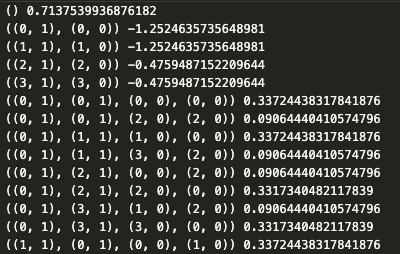
\includegraphics[width=0.3\textwidth]{/Users/choeyunho/Documents/mygit/2025_GBBD/실험코드_주석정리/fig/ham_int.png}
    \caption{molecular Hamiltonian}
    \label{fig:my_image}
\end{figure}
\begin{enumerate}[label=\textbf{*}, leftmargin=*]
  \item () : 가장 위의 공란은 Constant 값 (여기서는 핵간 척력) 
  \item ((0,1),(0,0)) : 튜플의 튜플로 정의 된다. 안의 튜플은 순서대로 (연산이 수행되는 오비탈 idx, 생성(1)인지, 소멸(0)인지) 결국 second Quantization 에서 1차여기항에 대응된다. 
  \item ((0, 1), (0, 1), (0, 0), (0, 0)) : 튜플 4개로 정의 된다. 안의 튜플은 위에서와 같은 정보를 사용. 결국 second Quantization 에서 2차여기항에 대응된다. 
\end{enumerate}

\subsection{(**) get\_fermion\_operator(ham\_int)}
1차, 2차 적분의 결과를 아래와같이 fermionic 생성/소멸 연산자의 표기법을 통해 2nd Quantized 해밀토니안으로 표현한다. 
\begin{figure}[H]
    \centering
    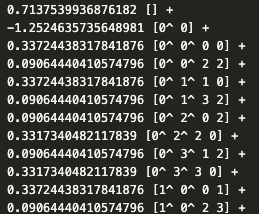
\includegraphics[width=0.3\textwidth]{/Users/choeyunho/Documents/mygit/2025_GBBD/실험코드_주석정리/fig/ham_fci.png}
    \caption{fermionic op}
    \label{fig:my_image}
\end{figure}
여기서, 
\begin{center}
[] : Constant 값 (여기서는 핵간 척력) 

[i\textasciicircum  j] : $a^{\dagger}_i a_j $ 

[i\textasciicircum  j\textasciicircum k l] : $a^{\dagger}_i a^{\dagger}_j a_k a_l $ 
\end{center}

\newpage

\subsection{(***) get\_number\_preserving\_sparse\_operator()}
아래와같이 희소행렬 표현으로 FCI 행렬을 구성한다. 
\begin{figure}[H]
    \centering
    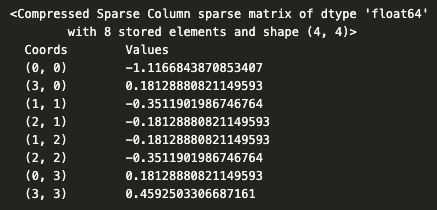
\includegraphics[width=0.8\textwidth]{/Users/choeyunho/Documents/mygit/2025_GBBD/실험코드_주석정리/fig/h_matrix.png}
    \caption{FCI matrix}
    \label{fig:my_image}
\end{figure}

\newpage

\section{FCI 행렬 -> 그래프로 변경}

\begin{CodeBox}[title={Example: Python snippet}]
def sparse_to_graph(A, *,
                    weight="value",   # "value" | "abs" | "binary"
                    symmetrize=True,  # 무향 그래프용: 패턴을 A + A.T로 합칠지
                    tol=0.0) :         # |a_ij|<=tol 은 0 취급
    """
    희소행렬 A -> NetworkX Graph/DiGraph 변환

    Parameters
    ----------
    A : scipy.sparse matrix (이경우 FCI 행렬)
    weight : {"value","abs","binary"}
        엣지 weight 설정 방법
        - "value": a_ij (실수/복소 가능; 복소는 실수부 사용 권장)
        - "abs"  : |a_ij|
        - "binary": 1 (연결만 표현)
    symmetrize : bool
        무향 그래프에서 A의 패턴을 A + A^T로 결합 (권장)
    tol : float
        임계값 이하 절댓값은 0으로 무시

    Returns
    -------
    G : nx.Graph 
    """

    # 그래프 에서 다루기 편햔 COO로 변환
    A = A.tocoo(copy=True)
    #COO 에서는 값을 아래와같이 3개의 어레이로 저장 
    #data : [3,4,2,7]
    #row : [0,0,1,3]
    #col : [2,4,1,3]
    #그리고 같은 인덱스 순서대로 0행 2열에는 3이라는 값이 있고 마찬가지로 총 4개의 원소가 있는 행렬을 표현한다. 

    # tol 필터링
    if tol > 0:
        mask = np.abs(A.data) > tol
        A = coo_matrix((A.data[mask], (A.row[mask], A.col[mask])), shape=A.shape)
    #0에 가깝지만 0이 아닌 원소에 대해 그 값을 0으로 만들기 위한 함수. 
    #

    # 대각 요소 처리
    if not keep_diagonal:
        mask = A.row != A.col
        A = coo_matrix((A.data[mask], (A.row[mask], A.col[mask])), shape=A.shape)

    # 무향이면 패턴 대칭화(권장): A <- A + A.T (중복은 합쳐짐)
    if not directed and symmetrize:
        AT = coo_matrix((A.data, (A.col, A.row)), shape=A.shape)
        A = (A + AT).tocoo()

    # 그래프 타입 선택
    G = nx.Graph()
    G.add_nodes_from(range(A.shape[0]))  # 노드: 0..n-1

    # weight 설정
    if weight == "binary":
        # 동일 (i,j) 중복 합치기 위해 집계
        from collections import defaultdict
        edges = defaultdict(float)
        for i, j, v in zip(A.row, A.col, A.data):
            if not directed and i == j and not keep_diagonal:
                continue
            key = (i, j) if directed else (min(i, j), max(i, j))
            edges[key] = 1.0  # 존재만 표시
        for (i, j), w in edges.items():
            G.add_edge(i, j, weight=w)

    else:
        # "value" 또는 "abs"
        if weight == "abs":
            vals = np.abs(A.data)
        elif weight == "value":
            # 복소인 경우 실수부만 쓰고 싶다면 .real 사용
            # 필요에 따라 변경 가능: vals = np.real(A.data)
            vals = A.data
        else:
            raise ValueError("weight must be 'value', 'abs', or 'binary'")

        # 동일 엣지 중복 합치기(무향일 때 i<j 묶기)
        from collections import defaultdict
        edges = defaultdict(float)
        for i, j, v in zip(A.row, A.col, vals):
            if not directed and i == j and not keep_diagonal:
                continue
            key = (i, j) if directed else (min(i, j), max(i, j))
            edges[key] += float(v)  # 누적(합). 필요시 max/mean 등으로 변경 가능.

        for (i, j), w in edges.items():
            G.add_edge(i, j, weight=w)

    return G
\end{CodeBox}

\section{main 에너지 계산 함수}

% 박스 안: 원문 코드만
\begin{CodeBox}[title={Example: Python snippet}]
def GBBD(mol):
  # 입력 : qiskit 의 molecularinfo 와 같이 분자의 정보를 담고있는 클래스인 MolecularData
  # 이후에 추가 설명
  mol = run_pyscf(mol, run_scf=1, run_fci=0)
  # 3. 2차 정량화 Hamiltonian 얻기
  ham_int = mol.get_molecular_hamiltonian()
  ham_fci = get_fermion_operator(ham_int)     
  #H = get_sparse_operator(ham_fci, n_qubits=mol.n_qubits)
  H = get_number_preserving_sparse_operator(
  fermion_op=ham_fci,
  num_qubits=mol.n_qubits,
  num_electrons=mol.n_electrons,       # 필수
  spin_preserving=True ,        # S_z 고정 (필요 없으면 None)
  reference_determinant=None,
  excitation_level=None)
  print(H)
  H_real = H.real
  G = sparse_to_graph(H_real, directed=False, weight="abs", symmetrize=True, tol=0.0)
  ccs = list(nx.connected_components(G))
  
  sub_mat_idx_g = list(ccs[0])
  H_sub_g = H[sub_mat_idx_g, :][:, sub_mat_idx_g]
  print(H_sub_g)
  eigval_g, eigvec = eigsh(H_sub_g, k=1, which='SA')
  E_g = eigval_g[0]
  
  sub_mat_idx_e = list(ccs[1])
  H_sub_e = H[sub_mat_idx_e, :][:, sub_mat_idx_e]
  print(H_sub_e)
  eigval_e, eigvec = eigsh(H_sub_e, k=1, which='SA')
  E_e = eigval_e[0]
  
  return E_g, E_e
\end{CodeBox}



\end{document}